\documentclass{article}
\usepackage[utf8]{inputenc}
\usepackage{tikz}
\usepackage[final]{listings}
\usepackage{xcolor}
\usepackage[
backend=biber,
style=alphabetic,
sorting=ynt
]{biblatex}
\addbibresource{bibo.bib}
\usepackage{pgfplots} 
\pgfplotsset{width=10cm,compat=1.9} 
\usepackage{chngcntr}
\counterwithin{figure}{section}

\title{Solving the Dynamic Predecessor Problem in Log-Logarithmic Time}
\author{Calvin Higgins 
\and Ethan Carlson 
\and Robert Oganesian}
\date{April 2022}

\begin{document}

\maketitle

\section{Abstract}
The dynamic predecessor problem consists of maintaining some dynamic ordered set $S_k$ on a bounded universe $U_k$. We solve this problem through a C++ implementation of Willard’s y-fast trie, a data structure that provides dynamic ordered set operations in log-logarithmic time. We provide some novel optimizations synthesized from several sources. Additionally, we engineer a testing suite, benchmarking suite and demo program.

\section{Preliminaries}

\noindent
Unfortunately, understanding the dynamic predecessor problem requires some level of mathematical formality: both to understand the literature and our implementation. To that end, we provide several definitions of terms used throughout the paper. We assume familiarity with binary strings. 
\\

\noindent
\textbf{Definition 1.1.} We define a bounded universe $U_k$ as $\{x\: |\: x \in {Z}, 0 \leq x < k\}$ for some ${k \geq 0}$. Intuitively, $U_k$ contains all non-negative integers from $0$ up to but not including $k$. For example, ${U_2 = \{0, 1\}}$ and ${U_4 = \{0, 1, 2, 3\}}$. We restrict bounded universes to non-negative integers both for simplicity and convenience. However, there is no reason the definition cannot be extended to the negative integers. 
\\

\noindent
\textbf{Definition 1.2.} We say a data structure $D$ is a set when $D$ provides a membership method. More concretely, data structure $D$ is set when $D$ has some method $contains(x)$ that returns $true$ if $D$ contains $x$ and $false$ otherwise. For example, if $D = \{0\}$ then $D.contains(0)$ is $true$ and $D.contains(1)$ is $false$.
\\

\noindent
\textbf{Definition 1.3.} A set $S$ is dynamic when $S$ provides update methods. More concretely, a set $S$ is a dynamic set if $S$ has some method $insert(x)$ which adds $x$ to the set and some method $remove(x)$ that removes $x$ from the set. For example, if $S = \{\}$ then after $S.insert(1)$, $S.insert(2)$ and $S.remove(2)$, $S = \{1\}$.
\\

\noindent
\textbf{Definition 1.4.} A set $S$ is ordered when $S$ provides predecessor and successor methods. More concretely, a set $S$ is a ordered set if $S$ has some method $predecessor(x)$ which returns the maximum $e \in S$ such that $e < x$ and $S$ has some method $successor(x)$ which returns the minimum $e \in S$ such that $e > x$. In the literature, $e \leq x$ and $e \geq x$ are used instead of $e < x$ and $e > x$, but these definitions are effectively equivalent \cite{10.1145/3409371}. For example, if $S = \{1, 3, 5\}$ then $S.predecessor(3) = 1$, $S.successor(3) = 5$ and $S.successor(4) = 5$. Additionally, we say that $S.predecessor(1)$ and $S.successor(5)$ are undefined.
\\

\noindent
\textbf{Definition 1.5} We say a set $S$ is on some bounded universe $U_k$ if $S$ stores only elements of $U_k$ and can store all elements of $U_k$. For convenience, we denote such a set as $S_k$ where $k$ is given by $U_k$. 
\\

\noindent
\textbf{Definition 1.6.} The dynamic predecessor problem entails implementing a dynamic ordered set $S_k$ on a bounded universe $U_k$ \cite{10.1145/3409371}. Some familiar data structures such as red-black trees solve the dynamic predecessor problem in logarithmic time. 

\section{Introduction}

\noindent
We aim to solve the dynamic predecessor problem in log-logarithmic time and linear space. To that end, we implement Willard's y-fast trie \cite{WILLARD198381}. This data structure splits the universe $U_k$ into partitions satisfying the dynamic ordered set operations. These partitions are stored in an index providing efficient look-up operations. We implement the partitions as red-black trees and the index as an x-fast trie. 
\\

\noindent
There are few high quality, open source implementations of these data structures. Therefore, we aim to provide a production-ready C++ implementation. We include benchmarking and testing suites to verify our implementation. Additionally, we provide an interactive y-fast trie as an educational resource.
\\

\section{Methods}
\subsection{Red-Black Tree}


\begin{figure}[ht]
    \centering
    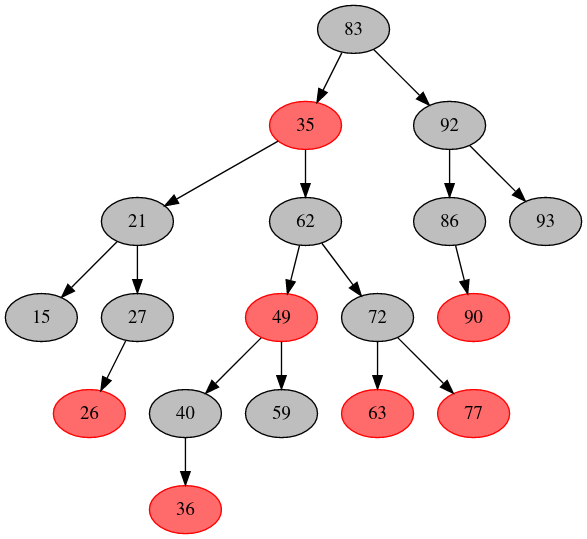
\includegraphics[height = 4cm]{examplerbtree.png}
    \caption{An example of a red black tree}
\end{figure}

\noindent
The purpose of the red-black tree, as implemented in this solution, is to do several set operations in $O(log(n))$ time, with $n$ in this context being used to represent the number of nodes in the red-black tree. These operations include insert, remove, predecessor, successor, maximum, minimum. Additionally, split and merge are implemented to run in $O(n)$ time. The main cause of the $O(log(n))$ time is the invariant of the red-black tree which causes it to balance out over time, maintaining a height that is less than $2*log(n+1)$. This is done by having each node be assigned a color, red or black, and having cases checked after insertion or removal depending on the color of various nearby nodes to see what must be done to maintain balance.
\\

\noindent
Before we discuss the methodology behind the red-black tree itself, we should first discuss two of the predecessors to the red-black tree, the binary search tree and the 2-4 tree (2-3-4 tree), and discuss the methodology behind their operations. In doing so, we can gain a more fundamental understanding of how the conclusions in the red-black tree were reached.
\\

\noindent
The binary search tree is the fundamental data structure on which the 2-4 tree and the red-black tree are built upon. The aim of this structure, and the derived structures, are to provide more efficient look-up and storing of elements in an ordered set, along with more efficient alteration of said set. With the binary search tree, it approaches this goal relatively simply.
\\

\begin{figure}[ht]
    \centering
    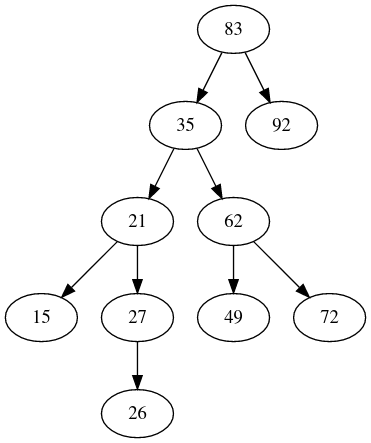
\includegraphics[height = 4cm]{bstexample.png}
    \caption{An example of a regular binary search tree}
\end{figure}

\noindent
In a binary search tree, each element is stored in a node. Each node has two children, in a left and right direction. The left child stores a key that is less than that of the parent node, the node which the children branch off of. Conversely, the right child stores a key greater than its parent’s. 
Given this relatively small set of rules, insertion, access and deletion are quite easily implemented.
\\

\noindent
Due to the results of binary insertion, and deletion maintaining those results, the tree may create a series of paths to each node that are shorter than a path containing all nodes in order. In the best case, the height of the tree, the length of the longest path from the root to a nil node, will be $log(n)$ rounded up. Unfortunately, given the simplicity of the structure’s rule set, this optimal result is far from guaranteed. An example of this is seen when a key greater than all existent keys is inserted into the tree repeatedly, causing the height of the tree being equal to the number of nodes in the tree. This, however, is far from the only example of a case causing imbalance. This is the same as having an ordered linked list, which does most set operations in $O(n)$ time. Thus, several data structures known as self balancing binary search trees were devised to amend this flaw, with a 2-4 tree being one of them.
\\

\begin{figure}[ht]
    \centering
    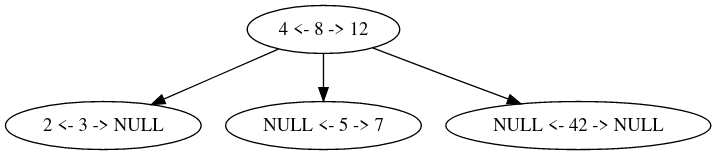
\includegraphics[width = 12cm]{24treeexample.png}
    \caption{An example of a 2-4 tree}
    \label{fig:my_label}
\end{figure}

\noindent
A 2-4 tree is a B-tree of order four, meaning that every node, instead of having one key and two children, can either have two, three or four children, with one, two or three keys. These keys are stored in the node in order, with the lesser keys being stored before the greater keys. Such nodes are referred to as 2-nodes, 3-nodes and 4-nodes respectively. Examples of each kind of node are shown below:
\\

\begin{figure}[ht]
    \centering
    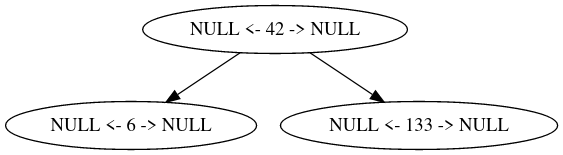
\includegraphics[width = 12cm]{2node.png}
    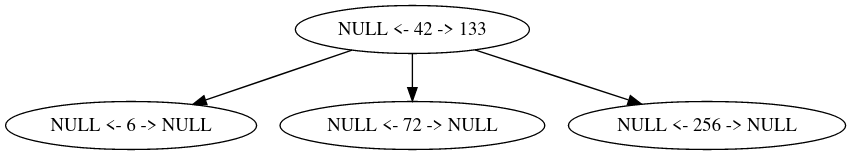
\includegraphics[width = 12cm]{3node.png}
    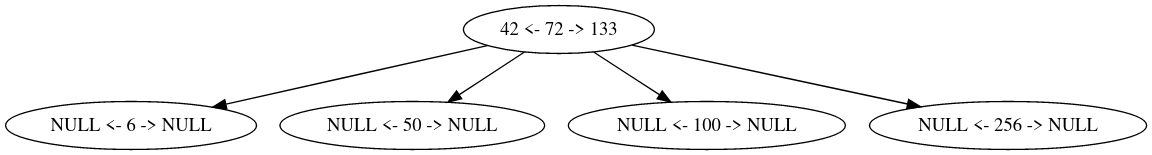
\includegraphics[width = 12cm]{4node.png}
    \caption{Examples of 2-4 tree nodes. In order from top to bottom, the examples are a 2-node, 3-node and a 4-node }
    
\end{figure}

\noindent
The amount of children is able to be only one more than the amount of keys because adjacent keys share one child. For example, a 3-node has three children. The leftmost child is the left child of the left key in the node, and the rightmost child is the right child of the right key in the node. However, the middle child of the node is both the right child of the left key in the node and the left child of the right key in the node. This makes sense intuitively, as the leftmost child is less than the left key, the rightmost child is greater than the right key, and the middle child is less than the right key and greater than left key.
\\

\noindent
Given that each node is equivalent to a binary search tree node with two children, the height of a 2-4 tree, when given the aforementioned scenario that makes the binary search tree inefficient, will have a height at least three times shorter than the binary search tree. However, this result alone does not create the desired property of self balance.
\\

\noindent
In order to achieve self balance, a set of rules were built on top of the process of binary search tree insertion and deletion that will distribute the keys around the tree in a relatively even fashion. In insertion, the process can be simply described as taking singular keys from the 4-nodes passed in traversal, distributing them upwards and outwards through the tree, and splitting the resulting 3-nodes into 2-nodes. This in turn creates self balance, as keys in more populated areas of the tree are transferred to less populated areas of the tree. However, this expansion of the binary tree creates a new problem, with that being the drastically increased complexity of the tree’s nodes, alongside the number of cases that must be considered in the operation of the tree. The creation of the red-black tree was a successful attempt to amend this problem \cite{rbtrees}.
\\

\noindent
Although red-black trees have vastly different appearances to 2-4 trees, they are actually isomorphic to each other. This means that a red-black tree can be mapped to a 2-4 tree with the same order of elements, and vise-versa. This begins to make sense when comparing the properties of the two structures.
\\

\noindent
As the name of the red-black tree suggests, each node is marked as either red or black. Such markings are done in accordance to the invariants of the red black tree, which are as follows:

\begin{itemize}
    \item The root of the red-black tree must be black
    \item Newly inserted nodes must be red
    \item There must not be a red node that has a red parent or any red children
    \item Each path of the tree must contain the same number of black nodes.
\end{itemize}

\noindent
With that covered, the parallel between the color of the red-black tree nodes and the multiple keys of the 2-4 tree nodes begins to form when the following is described: the red nodes are equivalent to the leftmost and rightmost keys of the 3-nodes and 4-nodes, and the black nodes are equivalent to the middle keys of all three types of 2-4 tree nodes. 
\\

\noindent
This parallel can be elaborated by comparing cases of subtrees in a  2-4 tree to subtrees of a red black tree. Thus, four pairs of parallel cases of subtrees from the two trees will be described and accompanied by a model to visualize the parallel below:
\\

\begin{figure}[h]
    \centering
    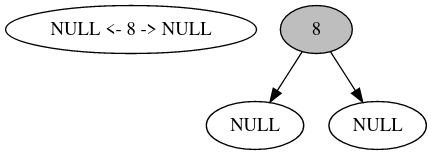
\includegraphics[width = 12cm]{8both.png}
    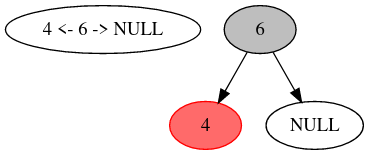
\includegraphics[width = 12cm]{46(both).png}
    \caption{Two examples of parallel subtrees of a red black and 2-4 tree}
\end{figure}

\begin{figure}[h]
    \centering
    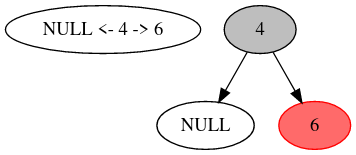
\includegraphics[width = 12cm]{4right6both.png}
    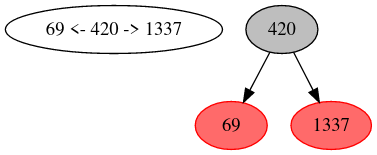
\includegraphics[width = 12cm]{694201337(both).png}
    \caption{Two more examples of parallel subtrees}
\end{figure}

\noindent
While the given parallel subtrees are far from comprehensive, it still holds that a pair of parallel subtrees can be created for every red-black subtree and 2-4 subtree, and thus the same applies for every red-black tree and 2-4 tree.
\\

\noindent
Given the parallels of the two data structures, one can correctly intuit that the criteria for restructuring a red black tree are parallel to the criteria for restructuring a 2-4 tree after a given operation; for the cases of the red black tree, one must simply replace the red-black subtree that is included in a given case with their corresponding 2-4 subtree. That said, one of the benefits of the red-black tree is that the cases are much simpler, as there are only two states of a red black tree: the node is red, or the node is black. Another benefit is that the nodes of  a red black tree are much simpler than a 2-4 tree, as the information of a red black tree node is as low as only one bit more than a binary search tree node, with that one bit being the color of the node. Of course, a red black tree is still much more complex than a binary search tree, requiring several cases for insertion and deletion on top of the cases already set by the binary search tree. The payoff for this is a guaranteed height that is less than 2*log(n+1).
\\

\subsection{X-Fast Trie}

\noindent
For simplicity, we assume that the x-fast trie is on the universe ${U_{2^4} = U_{16}}$. 
\\

\noindent
The x-fast trie is a bitwise trie stored in a tower of hash tables known as the level search structure.  
The bottom level of the level search structure contains the members of the x-fast trie. Each subsequent level contains prefixes from the level below it \cite{WILLARD198381}. For example, if $0101$ is a member of the x-fast trie, then the bottom level will contain $0101$. Also, the second lowest level will contain the prefix $010$, the third lowest level will contain the prefix $01$ and all subsequent levels will contain the prefix $0$ (see Figure 4.2.1). We only store $log_2(k) = log_2(2^4) = 4$ levels because any additional levels would be identical. Intuitively, this is because every length 4 binary string will be $0$ after $log_2(2^4) = 4$ prefix operations (equivalent to a single bitwise right shift).

\begin{center}
    \centering
    \textbf{Figure 4.2.1}\par\medskip
    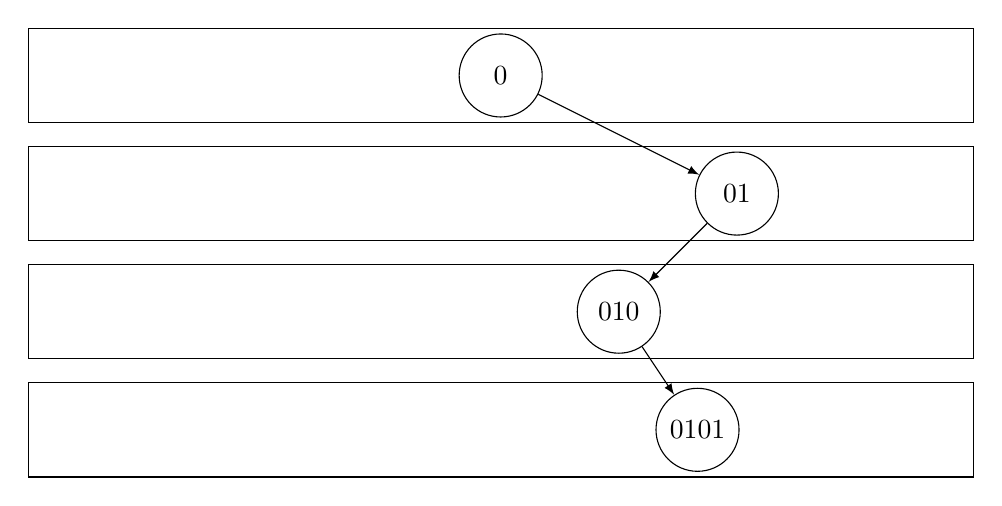
\begin{tikzpicture}[
            every node/.style = {minimum width = 3em, draw, circle},
            level/.style = {sibling distance = 60mm/#1},
            edge from parent/.style={draw,-latex}
        ]
       
        \node {0}
            child {edge from parent[draw = none] node[draw=none] {} 
                child {edge from parent[draw = none] node[draw = none] {}
                    child {edge from parent[draw = none] node[draw = none] {}}
                    child {edge from parent[draw = none] node[draw = none] {}}
                }
                child {edge from parent[draw = none] node[draw = none] {}
                    child {edge from parent[draw = none] node[draw = none] {}}
                    child {edge from parent[draw = none] node[draw = none] {}}
                }
            }
            child {node {01}
                child {node {010}
                    child {edge from parent[draw = none] node[draw=none] {}}
                    child {node {0101}}
                }
                child {edge from parent[draw = none] node[draw = none] {}
                    child {edge from parent[draw = none] node[draw = none] {}}
                    child {edge from parent[draw = none] node[draw = none] {}}
                }
        };
        \draw (-6,0.6) rectangle (6,-0.6);
        \draw (-6,-0.9) rectangle (6,-2.1);
        \draw (-6,-2.4) rectangle (6,-3.6);
        \draw (-6,-3.9) rectangle (6,-5.1);
    \end{tikzpicture}
    The level search structure of an x-fast trie on $U_{16}$ containing $0101$
\end{center}

\noindent
In order to improve space complexity, the nodes of the bitwise trie are conditionally stored in the level search structure. Leaf nodes are always stored because they represent set members. Internal nodes with 1 or 2 children are always stored while nodes with 0 children are never stored. The number of children of an internal node is the number of ways the node's prefix can be formed \cite{WILLARD198381}. For example, if the x-fast trie only contains $0101$ then the node with prefix $010$ on the second lowest level will have 1 child (see Figure 4.2.1). If the x-fast trie also contains $0100$, then the same node will have 2 children because the prefixes of $0100$ and $0101$ are both $010$ (see Figure 4.2.2). In the worst case, each additional member requires $O(log(k))$ space because a new prefix node must be created on each level of the level search structure. Therefore, the x-fast trie takes $O(n*log(k))$ space.
\\

\begin{center}
    \centering
    \textbf{Figure 4.2.2}\par\medskip
    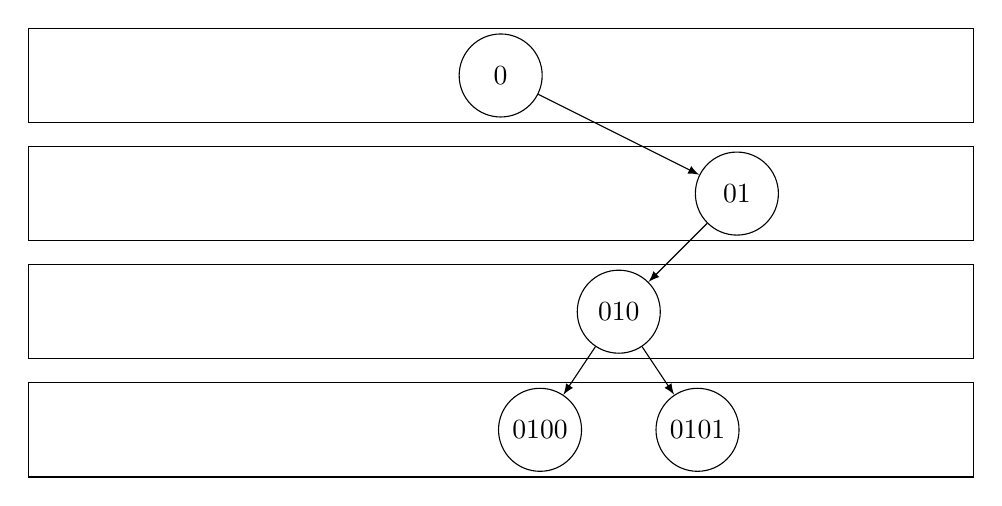
\begin{tikzpicture}[
            every node/.style = {minimum width = 3em, draw, circle},
            level/.style = {sibling distance = 60mm/#1},
            edge from parent/.style={draw,-latex}
        ]
        \node (A1) {0}
            child {edge from parent[draw = none] node[draw=none] (B1) {} 
                child {edge from parent[draw = none] node[draw = none] (C1) {}
                    child {edge from parent[draw = none] node[draw = none] (D1) {}}
                    child {edge from parent[draw = none] node[draw = none] (D2) {}}
                }
                child {edge from parent[draw = none] node[draw = none] (C2) {}
                    child {edge from parent[draw = none] node[draw = none] (D3) {}}
                    child {edge from parent[draw = none] node[draw = none] (D4) {}}
                }
            }
            child {node (B2) {01}
                child {node (C3) {010}
                    child {node (D5) {0100}}
                    child {node (D6) {0101}}
                }
                child {edge from parent[draw = none] node[draw = none] (C4) {}
                    child {edge from parent[draw = none] node[draw = none] (D7) {}}
                    child {edge from parent[draw = none] node[draw = none] (D8) {}}
                }
        };
        \draw (-6,0.6) rectangle (6,-0.6);
        \draw (-6,-0.9) rectangle (6,-2.1);
        \draw (-6,-2.4) rectangle (6,-3.6);
        \draw (-6,-3.9) rectangle (6,-5.1);
    \end{tikzpicture}
    The level search structure of an x-fast trie on $U_{16}$ containing $0100$ and $0101$
\end{center}

\noindent
The bitwise trie stored in the level search structure is also threaded. This means that each missing right pointer points to the largest member in the subtree and each missing left pointer points to the smallest member in the subtree (see Figure 4.2.3) \cite{WILLARD198381}. We call these pointers skip links. Skip links enable shortcuts from certain internal nodes to certain leaf nodes. With some thought, it becomes evident that for each non-member of the x-fast trie, the internal node with the longest matching prefix with that non-member must have a skip link. 
\\

\begin{center}
    \centering
    \textbf{Figure 4.2.3}\par\medskip
    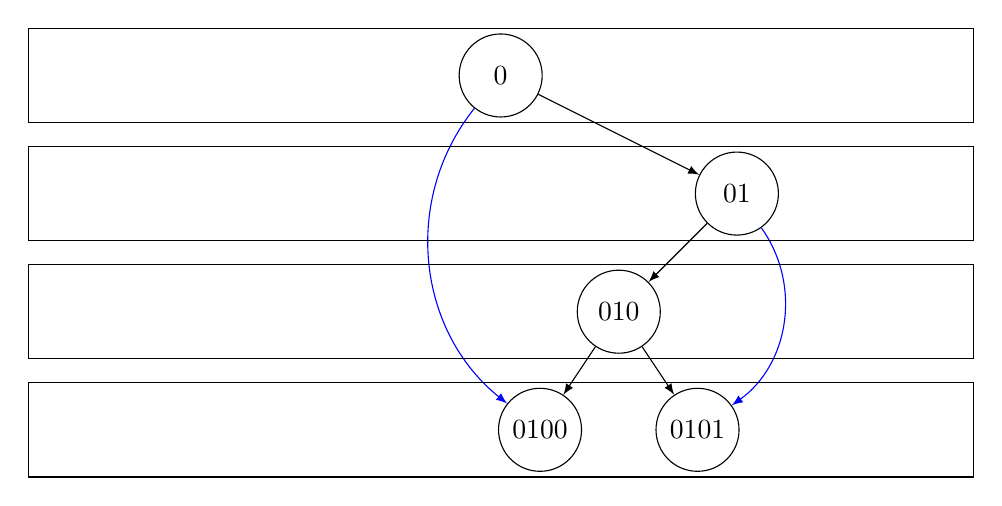
\begin{tikzpicture}[
            every node/.style = {minimum width = 3em, draw, circle},
            level/.style = {sibling distance = 60mm/#1},
            edge from parent/.style={draw,-latex}
        ]
        \node (A1) {0}
            child {edge from parent[draw = none] node[draw=none] (B1) {} 
                child {edge from parent[draw = none] node[draw = none] (C1) {}
                    child {edge from parent[draw = none] node[draw = none] (D1) {}}
                    child {edge from parent[draw = none] node[draw = none] (D2) {}}
                }
                child {edge from parent[draw = none] node[draw = none] (C2) {}
                    child {edge from parent[draw = none] node[draw = none] (D3) {}}
                    child {edge from parent[draw = none] node[draw = none] (D4) {}}
                }
            }
            child {node (B2) {01}
                child {node (C3) {010}
                    child {node (D5) {0100}}
                    child {node (D6) {0101}}
                }
                child {edge from parent[draw = none] node[draw = none] (C4) {}
                    child {edge from parent[draw = none] node[draw = none] (D7) {}}
                    child {edge from parent[draw = none] node[draw = none] (D8) {}}
                }
        };
        \path (A1) edge[bend right=45, color=blue, draw, -latex] (D5);
        \path (B2) edge[bend left=45, color=blue, draw, -latex] (D6);
        \draw (-6,0.6) rectangle (6,-0.6);
        \draw (-6,-0.9) rectangle (6,-2.1);
        \draw (-6,-2.4) rectangle (6,-3.6);
        \draw (-6,-3.9) rectangle (6,-5.1);
    \end{tikzpicture}
    The level search structure with skip links colored blue.
\end{center}

\noindent
Suppose an internal node with 2 children has a matching prefix with a given non-member. Then, if the non-member was in the x-fast trie, then the non-member would either be in the left subtree or in the right subtree of the internal node. If a non-member would have been in an subtree, then the root node of that subtree must have a matching prefix. Therefore, either the root of the left subtree or the root of the right subtree must have a longer matching prefix than the given internal node. This shows that no internal node with 2 children can have the longest matching prefix. Therefore, the internal node with the longest matching prefix must have a skip link. 
\\

\noindent
Following this skip link, we will either find the predecessor or the successor of the non-member. Therefore, either the predecessor or the successor of a non-member can be found by searching for the internal node with the longest matching prefix then following the skip link. The predecessor will be found if the skip link is on the right and the successor will be found if the skip link is on the left. By storing the bottom level in a linked list, the successor can be found from the predecessor and vice versa \cite{WILLARD198381}.
\\

\noindent
For example, consider finding the successor of 0111 when the x-fast trie contains 0100 and 0101. The internal node with the longest matching prefix is 01 on the second highest level. Following the right skip link, we find that the successor of 0111 is 0101.
\\

\begin{center}
    \centering
    \textbf{Figure 4.2.3}\par\medskip
    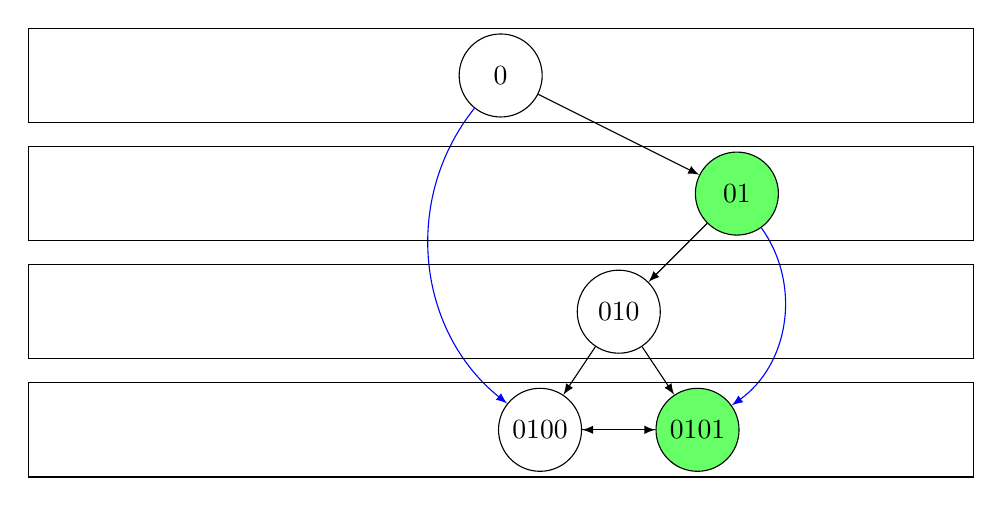
\begin{tikzpicture}[
            every node/.style = {minimum width = 3em, draw, circle},
            level/.style = {sibling distance = 60mm/#1},
            edge from parent/.style={draw,-latex}
        ]
        \node (A1) {0}
            child {edge from parent[draw = none] node[draw=none] (B1) {} 
                child {edge from parent[draw = none] node[draw = none] (C1) {}
                    child {edge from parent[draw = none] node[draw = none] (D1) {}}
                    child {edge from parent[draw = none] node[draw = none] (D2) {}}
                }
                child {edge from parent[draw = none] node[draw = none] (C2) {}
                    child {edge from parent[draw = none] node[draw = none] (D3) {}}
                    child {edge from parent[draw = none] node[draw = none] (D4) {}}
                }
            }
            child {node[fill=green!60] (B2) {01}
                child {node (C3) {010}
                    child {node (D5) {0100}}
                    child {node[fill=green!60] (D6) {0101}}
                }
                child {edge from parent[draw = none] node[draw = none] (C4) {}
                    child {edge from parent[draw = none] node[draw = none] (D7) {}}
                    child {edge from parent[draw = none] node[draw = none] (D8) {}}
                }
        };
        \path (A1) edge[bend right=45, color=blue, draw, -latex] (D5);
        \path (B2) edge[bend left=45, color=blue, draw, -latex] (D6);
        \path (D5) edge[draw, -latex] (D6);
        \path (D6) edge[draw, -latex] (D5);
        \draw (-6,0.6) rectangle (6,-0.6);
        \draw (-6,-0.9) rectangle (6,-2.1);
        \draw (-6,-2.4) rectangle (6,-3.6);
        \draw (-6,-3.9) rectangle (6,-5.1);
    \end{tikzpicture}
    The longest matching prefix and successor are colored green.
\end{center}

\noindent
Therefore, we only need to find the internal node with the longest matching prefix to find both the predecessor and successor. Through linear search, this node can be found in $O(log(k))$ time. However, by viewing the level search structure as a monotone sequence of 0s and 1s, that is, a sequence of 0s followed by a sequence of 1s, this node can be found in $O(log(log(k))$ time. A level is considered 1 if the level contains a matching prefix and considered 0 otherwise. The level containing the longest matching prefix is given by the first 1 in the sequence. By binary searching for the 0 to 1 transition, the longest matching prefix can be found in $O(log(log(k))$ time \cite{WILLARD198381}. From there, the predecessor and successor can be found in constant time.
\\

\noindent
However, maintaining both the level search structure and the threaded bitwise trie under updates is challenging. First, consider insertion. The new leaf node must be inserted into the linked list on the bottom of the level search structure. To do this, the predecessor and successor of the new leaf node must be known. Then, the internal nodes need to be updated. Traversing down the bitwise trie from the root node, we must create missing internal nodes from the prefixes of the new member. Additionally, when we encounter a node with a skip link that we do not replace with an internal node, we may need update that skip link. If the skip link is on the right and the new leaf node is greater than the current skip link, then the skip link should point to the new leaf. Otherwise, if the skip link is on the left and the new leaf node is less than the current skip link, then the skip link should point to the new leaf. Clearly, only the roots of subtrees containing the new leaf node need to be updated. We traverse through these nodes, updating skip links only if the insertion has changed the minimum or maximum of the subtree. This is because all skip links either point to the minimum value of the subtree or the maximum value of the subtree. Clearly, this algorithm takes $O(log(k))$ time because we must traverse the entire height of the trie.
\\

\noindent
Now, consider removal. The leaf node must be removed from the linked list on the bottom of the trie. Working from the bottom up, internal nodes with 0 children must be removed and skip links to the removed leaf node must be updated. Recall that skip links can only go to leaf nodes, so we only need to update skip links to the removed node since no other skip links will have changed. In fact, skip links to the removed leaf node only need to be set to either the predecessor or the successor of the removed leaf. For right skip links, this is because if the predecessor is not in the subtree of the node to be updated, then the subtree of the node must be empty and therefore, the node will have 0 children and will be removed. A similar argument holds for left skip links and the successor. Therefore, we avoid an expensive predecessor and successor search on each level. This provides a time complexity of $O(log(k))$ instead of $O(log^2(k))$.
\\

\subsection{Y-Fast Trie}

\noindent
The y-fast trie improves the time and space complexity of the x-fast trie by adding a layer of indirection  \cite{WILLARD198381}. Instead of storing members directly in the x-fast trie, they are stored in red-black trees. These red-black trees split the universe into $O(log(k))$ sized partitions and are stored in an x-fast trie. The x-fast trie functions as an index, allowing partitions to be accessed $O(log(log(k)))$ time. Once partitions are found, dynamic ordered set operations can be performed in $O(log(log(k)))$ time because partitions only contain $O(log(k))$ members. However, updates to the index must happen with low probability or the $O(log(k))$ update complexity of x-fast trie will dominate the analysis.
\\

\noindent
Therefore, we insert into the x-fast trie only after at least $log(k)$ insertions. In the worst case, after $log(k)$ insertions into partitions that containing $log(k)$ members, a partition could have $2*log(k)$ members. To maintain the $O(log(k))$ size of this partition, we split it in half in $O(log(log(k)))$ time and insert two new partitions into the x-fast trie in $O(log(k))$ time. However, this update only happens with $O(1/log(k))$ probability. Therefore, on average, the cost of inserting into the x-fast trie is $O(1)$. The upper bound of $2*log(k)$ on the partition size is an arbitrary parameter. As long as the coefficient on the maximum partition size is greater than 1, this analysis will hold. For example, considering partitions too large when they have $8*log(k)$ members still works.
\\

\noindent
Like insertion, we remove from the x-fast trie only after at least $log(k)$ removals. In the worst case, after $log(k)$ removals from partitions containing $log(k)$ members, one partition could have $0$ members. To maintain the space complexity of the y-fast trie, we remove the partition from the x-fast trie in $O(log(k))$ time. However, this update only happens with $O(1/log(k))$ probability. Therefore, on average, the cost of removing from the x-fast trie is $O(1)$. The lower bound of $0$ on the partition size is an arbitrary parameter. As long as the coefficient on the minimum partition size is less than 1, this analysis will hold. For example, considering partitions too small when they have $\frac{1}{2}*log(k)$ members still works. In this case, the too small partition is merged with an adjacent partition and then split if the merged partition is too large, instead of simply removing the partition.
\\

\noindent
Clearly, the partitions stored in the x-fast trie must provide some information about their bounds. The bounds of the partition are indicated by a representative value \cite{WILLARD198381}. We will consider two possible representative schemes. In both schemes, the representative is the maximum possible value in the partition.
\\

\noindent
In the first scheme, the set of possible representatives is predetermined and each member has a closest representative. The closest representative is the smallest representative such that it is less than or equal to the member. We choose these representatives so they occur exactly $log(k)$ apart. This ensures that when all partitions are full, they will have exactly $log(k)$ members each.  
\\

\noindent
For example, with $U_{16}$ the possible representatives are 3, 7, 11 and 15. Suppose we have a y-fast trie on $U_{16}$ and we insert 6. Then, the representative of 6, which is 7, will be inserted into the x-fast trie along with a red-black tree containing 6. Now, suppose we insert 0. Since the representatives only indicate the upper bound of the partition and not the lower bound, 0 will be inserted into the existing partition. However, if we try to insert 8, we would have to create a new partition because 8 falls outside the bounds of any existing partitions. 
\\

\noindent
In the second scheme, the set of possible representatives is not predetermined but each member still has a closest representative. The closest representative is the smallest representative such that it is less than or equal to the member. When a new partition is inserted, the representative of the partition is the first value inserted into it.
\\

\noindent
For example, suppose we have a y-fast trie on $U_{16}$ and we insert 6. Then, when 6 is inserted, a partition with representative of 6 will be created. Now, suppose we insert 0. Since the representatives only indicate the upper bound of the partition and not the lower bound, 0 will be inserted into the existing partition. However, if we try to insert 8, we would have to create a new partition because 8 falls outside the bounds of any existing partitions. 
\\

\noindent
The correct partition for a given member is the inclusive successor of the member's representative in the x-fast trie. This can be found in $O(log(log(k)))$ time. Then, the predecessor and successor of the member in the y-fast trie may be computed in an additional $O(log(log(k)))$ operation on the partition. 

\section{Implementations}
\subsection{Red-Black Tree}


\noindent
This section serves to give details of the core methods included in the red black tree. This will be done in two subsections, subsection 5.1.1 and subsection 5.1.2. 5.1.1 will cover the procedure and result of the method, while 5.1.2 will cover details specific to our implementation of these methods in the red black tree, usually those that are deemed to be noteworthy. It should be noted that not all methods of the red black tree will be covered, namely those that are private and thus irrelevant to the user, as well as those that are for debugging or visualization.
\\

\subsubsection{Method Descriptions}

\paragraph{Contains}

\noindent
Contains returns true if the input key is inside of the tree, and false if otherwise. The body of this method is one line, as it simply calls the find method, which returns the node in the tree containing the input key, or a null pointer if said node does not exist, and checks if the return value is not a null pointer. Thus, it is best to cover the find method instead, as it is used in several places apart from contains as well. The find method, and by extension the contains method, run with a time complexity of $O(log(n))$
\\

\noindent
The find method works as follows:

\begin{itemize}
    \item Make a target node, and set it to the root of the tree.
    \item While the target node is not a null pointer, and the key of the target node is not equal to the input, set the target node to the right child if the input is greater than the key of the target node, or the left child if otherwise.
    \item Return the target node, which could be a null pointer.
\end{itemize}

\noindent
The pseudocode described above does not serve the actual implementation very well, so the actual implementation will be described in the section covering the noteworthy details of the implementations of each method.
\\

\paragraph{Insert}

\noindent
Insertion puts a new node into the red-black tree with a given value in $O(log(n))$ time. It does this by performing a standard binary search tree insertion, and then enforcing the red-black tree invariant afterwards. Additionally, the min and max of the tree are updated if a new min/max is added to the tree. Binary search tree insertion works by starting at the root of the tree, and comparing the targeted node’s key with the key to be inserted, which determines which direction it will go in the traversal. It does this until a null pointer is found, or a duplicate key is found. If it finds a null pointer, the key will be inserted. If it finds that the key is already in the tree, the insertion will be canceled. When inserted, the node’s color starts as a red node, but may be changed. After the insertion, there are four cases that will be checked to determine what must be done in order to maintain the invariant. The cases are as follows:
\\

\noindent
Case 1: The inserted node is the root of the tree. If so, then simply recolor the node black.
\\

\noindent
Case 2: The inserted node has a black sibling. If so, do a rotation on the parent and possibly the grandparent depending on if the parent and child are both in the same direction relative to their parents. Afterwards, the colors of the parent and its children are swapped. The direction of the rotation also depends on the aforementioned relative direction.
\\

\noindent
Case 2.1: If the parent goes in a different direction than the grandparent, then do a rotation on the parent in the direction opposite of the direction the inserted node goes in. Afterwards, do a rotation on the grandparent in the direction that the inserted node goes in.
\\

\noindent
Case 2.2: If the parent goes in the same direction as the grandparent, then do a rotation on the grandparent in the direction the inserted node goes in. 
\\

\noindent
Case 3: The inserted node has a red sibling. If so, then recolor the cousins of the node.
\\

\noindent
Case 4: On top of the conditions of case 3, if the grandparent of the inserted node is not the root, then inverse the color of the grandparent and recall the insertion check on the grandparent. Also, ensure the root color is black.
\\

\paragraph{Remove}

\noindent
Remove takes out a given key from the tree in $O(log(n))$ time. It does this by following the binary search tree deletion first, and then doing a procedure which maintains the invariant of the red-black tree. Additionally, if the removed node is either the min or the max, it is updated to be the successor of the min or the predecessor of the max respectively. Binary search tree deletion works according to 6 cases, which are as follows:
\\

\noindent
Case 1: The targeted node is a leaf, so delete it without further action.
\\

\noindent
Case 2: The targeted node has only a right child, so replace the targeted node with it before deleting the target node.
\\

\noindent
Case 3: The targeted node has only a left child. If so, replace the targeted node with its child before deleting the target node.
\\

\noindent
Case 4: The targeted node has two children. If so then replace the node’s key with the key of its successor. Then, delete the successor instead of the target node.
\\

\noindent
Case 5: The targeted node is the root and has two children. If so, then follow case 4.
\\

\noindent
Case 6: The targeted node is the root and has one child. If so, replace the root with its only child.
\\

\noindent
Cases 5 and 6 may seem slightly redundant, but they are considered to be different cases due to their implementation in the code. This is because cases 1 through 4 have interactions with the parent node without checking if it is null for the sake of optimization. Thus, cases 5 and 6 need to be separated in order to avoid a segmentation fault.
\\

\noindent
After the standard binary search tree deletion is performed, a potentially recursive call must be made to maintain the red black tree invariant after deletion. In this call, there are 6 cases that are checked, each with a certain protocol afterwards. These cases are as follows and are checked in that order, with previous cases not being acted upon unless stated otherwise:
\\

\noindent
Case 1: The color of the deleted node is red. If so, just color the parent of the deleted node black.
\\

\noindent
Cases 2-6: The deleted node is black. If so, then recolor its sibling red if it exists.
\\
\noindent
Case 2: The deleted node was black, but the parent was red. If so, just recolor the parent black.
\\

\noindent
Case 3: The deleted node was black, but the parent was the root. If so, then there would not be a black height problem once the sibling is recolored red, so do nothing.
\\

\noindent
Case 4: The deleted node has a sibling, so swap the color of the parents and sibling, and then rotate about the parent in the direction that the deleted node goes in. Afterwards, run the parent through the deletion cases.
\\

\noindent
Case 5: The child of the parent’s sibling in the direction of the parent is red and the other child of the parent’s sibling is black or null. If so, swap the color of the parent's sibling and its red sibling, and do a rotation in the direction opposite of the parent on the parent's sibling.
\\

\noindent
Case 6: After case 5, the parent's sibling is now black. If so, then swap colors between the parent's sibling and the parent's parent. Then do a rotation in the parent's direction on the deleted node's grandparent.
\\

\paragraph{Predecessor}

\noindent
Predecessor returns the key in the tree that is strictly lower than the input key. The input key does not have to be in the tree. If there is no key in the tree strictly lower than the input key, then a null value has to be returned. Thus, the method returns the key in an std::optional so that this can be done. The run-time for this method has a time complexity of $O(log(n))$
\\

\noindent
The code for this works as so:

\begin{itemize}
    \item If the tree is empty, return null
    \item Make a node variable (we will call it target 1), and set it to root.
    \item While target 1 has a child with a key that is less than the input, set target 1 to that child. If a key equal to the input is found in this process, stop the process prematurely
    \item If the key of target 1 is now greater than the input, return target 1’s key.
    \item Make a new node variable(we will call it target 2), and set it to the right child of target 1.
    \item While target 2 has a left child, set target 2 to its left child. Once there is no longer a left child, return target 2.
    \item Set target 2 to target 1’s parent.
    \item While target 2 is not a null pointer, and target 1 is not the left child of target 2, set target 1 to target 2 and set target 2 to its own parent.
    \item If target 2 is not a null pointer, return its key. If not, return null.
\end{itemize}

\noindent
The result of this pseudocode can be described as this:

\begin{itemize}
    \item If the tree is empty, then return nothing.
    \item If the node that has the key closest to the input is less than the input, return that key.
    \item If the aforementioned node has a left child, then return the in-order predecessor of that node. The in-order predecessor would be the rightmost descendant of the left child, or the left child if the left child has no right child.
    \item If the aforementioned node has no left child, then traverse up the tree until the second to last node in the upwards traversal is a right child, or the last node traversed was a null pointer.
    \item If the last node in the traversal was not a null pointer, return that node. Otherwise, return nothing.
\end{itemize}

\paragraph{Successor}

\noindent
Successor returns the key in the tree that is strictly greater than the input key. The input key does not have to be in the tree. If there is no key in the tree strictly greater than the input key, then a null value has to be returned. Thus, the method returns the key in an std::optional so that this can be done. The run-time for this method has a time complexity of $O(log(n))$
\\

\noindent
The code for this works as so:

\begin{itemize}
    \item If the tree is empty, return null
    \item Make a variable to store a target node (we will call it target 1), and set it to root.
    \item While target 1 has a child with a key that is greater than the input, set target 1 to that child. If a key equal to the input is found in this process, stop the process prematurely
    \item If the key of target 1 is now less than the input, return target 1’s key.
    \item Make a new target variable (we will call it target 2), and set it to the left child of target 1.
    \item While target 2 has a left child, set target 2 to its right child. Once there is no longer a right child, return target 2.
    \item Set target 2 to target 1’s parent.
    \item While target 2 is not a null pointer, and target 1 is not the left child of target 2, set target 1 to target 2 and set target 2 to its own parent.
    \item If target 2 is not a null pointer, return its key. If not, return null.
\end{itemize}

\noindent
The result of this pseudocode can be described as this:

\begin{itemize}
    \item If the tree is empty, then return nothing.
    \item If the node that has the key closest to the input is greater than the input, return that key.
    \item If the aforementioned node has a right child, then return the in-order successor of that node. The in-order successor would be the leftmost descendant of the right child, or the right child if the right child has no left child.
    \item If the aforementioned node has no right child, then traverse up the tree until the second to last node in the upwards traversal is a left child, or the last node traversed was a null pointer.
    \item If the last node in the traversal was not a null pointer, return that node. Otherwise, return nothing.
\end{itemize}


\paragraph{Max and Min}

\noindent
Max returns the largest key stored in the tree, which can be nothing if the tree is empty, meaning it is returned using std::optional. Due to the invariant of binary search trees, the implementation of max is rather simple. The max of the tree will always be the rightmost node in the tree, which can potentially be the root of the tree. That said, one can use that fact to find the max with $O(log(n))$ time complexity by following this procedure:
\\

\begin{itemize}
    \item Make a node variable (we will call it n), and set it to the root of the tree.
    \item While n has a right child, set n to its right child.
    \item Return the key of n.
\end{itemize}

\noindent
While this operation is rather fast, it can be done faster if one makes the maximum of the tree an invariant that is maintained during insertion and removal. The result of this is that the maximum can be found in O(1) time, at the cost of a slight increase in the constant time of insertion and removal. It should be noted that maximum is stored as the node containing the maximum key in order to quickly maintain the invariant. In the description of the implementation, the variable containing the maximum node will be referred to as max.
\\

\noindent
During insertion, one must make the following checks:

\begin{itemize}
    \item If the inserted node is the only node in the tree, set max to that node.
    \item If the newly inserted node has a value greater than max, set max to that node.
\end{itemize}

\noindent
During deletion, one must make the following checks:
\begin{itemize}
    \item If there is a max, and the deleted node is max, then do one of the following:
    \item If max has a parent, then set max to its parent
    \item Otherwise, set max to its left child, which may be a null pointer. It is only a null pointer when max is the only node in the tree.
\end{itemize}

\noindent
Due to max being an invariant, a call to the max method simply returns the key of max, which, as stated, before is done with O(1) time complexity.
\\

\noindent
Min has a process identical to this, with the sole exception being that the uses of greater than and less than are reversed. Thus, min also runs in constant time.
\\

\paragraph{Get}

\noindent
Get returns the nth key of the tree’s set, with n being the number input into the method. This is done with O(n(log(n))) time complexity. Because the tree is not guaranteed to have any values, the return type is an std::optional. If n is greater than or equal to the size of the tree’s set (out of bounds), then the maximum value of the tree’s set is returned instead.
\\

\noindent
The procedure for out implementation of get is as follows:

\begin{itemize}
    \item If n is greater than or equal to the size of the tree, do one of the following:
        \begin{itemize} \item If there is a maximum node stored in the tree, then return its key. \end{itemize}
    \item Otherwise, return nothing.
    \item Make a node variable (we will call it $target$), and store the minimum node in it.
    \item Do the following n - 1 times:
        \begin{itemize}\item Set $target$ to the successor node of $target$. \end{itemize}
    \item Return the key of $target$.
\end{itemize}

\noindent
It should be noted that the O(nlog(n)) time complexity is due to calling an $O(log(n))$ operation, successor node, n times.
\\

\paragraph{Median}

\noindent
Median simply calls get with n set to the size of the tree divided by two. Because size is an invariant maintained during insertion and removal like max and min, size is found in O(1) time. Thus, median shares the time complexity of get, which is O(nlog(n)).
\\

\paragraph{Merge}

\noindent
The merge operation takes in nodes from the two input trees using in-order traversal, and then recursively forms subtrees from all of the nodes using an algorithm similar to merge sort. When doing this, it also keeps track of the deepest depth traversed, stores nodes that are at that depth, and then recolors of them red. All other nodes are colored black in the process. In effect, the result of the merge is a perfectly balanced tree from all nodes, with all but the leaves being colored black. The two original trees have their roots set to a null pointer afterwards, effectively making them empty. The nodes are reused, so proper deletion needs not be done. Due to all nodes only being traversed once, the algorithm runs with $O(n)$ time complexity.

Unfortunately, this algorithm only works when the first input tree has nodes that are all less than the nodes of the second tree.
\\

\paragraph{Split}

\noindent
The split operation simply puts the nodes from the input tree using in-order traversal into a vector, splits the vector into two subvectors, with the first containing all nodes from the left subtree, and the second containing the others, and then uses merge to create two trees from those two subvectors. The two trees are returned after creation, and the original tree has its root marked as a null pointer. As an extension to the merge algorithm, this algorithm also runs in $O(n)$ time.
\\


\subsubsection{Noteworthy Details of Method Implementation}

\noindent
One detail about our implementation of the red-black tree that is prevalent throughout much of the code is “branchless” procedures. These branchless procedures avoid the use of if else statements, typically by indexing into an array of predefined choices. An example can be seen below in our implementation of find:
\\

\begin{lstlisting}[language=C++,basicstyle=\tiny]
node_ptr find(key_type key){
    auto target_node = root_;
    while (target_node != nullptr && target_node->key_ != key) {
        target_node = target_node->children_[key > target_node->key_];
    }
    return target_node;
};
\end{lstlisting}

\noindent
Note that the array $children\_$ contains two node pointers, with the first being the left child of the parent, and the second being the right child.
\\

\noindent
Without branching, our find would look something like this:

\begin{lstlisting}[language=C++,basicstyle=\tiny]
node_ptr find(key_type key){
        auto target_node = root_;
        while (target_node != nullptr && target_node->key_ != key) {
            if(key > target_node->key_){
                target_node = target_node->children_[1];
            }
            else{
                target_node = target_node->children_[0];
            }
        }
        return target_node;
};
\end{lstlisting}

\noindent
Branchless code not only reduced the size of the source code where it was used, but it may also boost performance. Our testing was limited, as it would require the implementation of branched versions of complex functions, as well as an implementation of the node class that does not use a children array.
\\

\noindent
On the topic of optimizations, there are several methods that can be optimized in our red black tree. For instance, merge can be optimized to run with $O(log(n))$ time complexity if an invariant is added such that the black height of all subtrees are stored. If this version of merge was implemented, split could run in $O(log(n))$ by using merge \cite{rbtreejoin}
\\

\noindent
Unfortunately, implementing the invariant mentioned above proved to be out of the scope of our project, due to the dynamic cases that maintain the red black tree invariant.
\\

\subsection{X-Fast Trie}

\noindent
We implement the x-fast trie as a C++ class template specializing on unsigned integer types. The bounded universe is given by the size of the unsigned integer type. For example, with an unsigned 8 bit integer, the universe would be $U_{2^8}$ = $U_{256}$. Additionally, if the class template specialization is not meaningful, the code will refuse to compile.

\subsubsection{Set Operations}
As discussed in Section 4.2, the members of the x-fast trie are stored in the bottom of the level search structure. Therefore, we implement $contains(x)$ as a hash table look-up into the bottom level.

\begin{lstlisting}[language=C++,basicstyle=\small]
inline bool contains(key_type key) const noexcept {
	return lss_.back().contains(key);
}
\end{lstlisting}

\subsubsection{Ordered Set Operations}

\noindent
As discussed in Section 4.2, the node with the longest matching prefix can be computed in $O(log(log(k)))$ time through binary search on the level search structure.

\begin{lstlisting}[language=C++,basicstyle=\small]
size_type get_lmp_level(key_type key) const noexcept {
	size_type low_level = 0;
	size_type high_level = bit_length();

	while (low_level <= high_level) {
		auto mid_level = (low_level + high_level) / 2;
		auto prefix = get_prefix(key, mid_level);
		if (lss_.at(mid_level).contains(prefix)) 
			low_level = mid_level + 1;
		else 
			high_level = mid_level - 1;
	}

	return low_level - 1;
}
\end{lstlisting}

\noindent
Then, we can compute a leaf node that is either the predecessor or the successor by following the skip link from the longest matching prefix node. We must be careful to handle the case where the longest matching prefix node is a leaf node. This happens when the value to search for is a member of the trie.

\begin{lstlisting}[language=C++,basicstyle=\small]
node_ptr get_close_leaf(key_type key) const noexcept {
	auto lmp_level = get_lmp_level(key);
	auto prefix = get_prefix(key, lmp_level);
	auto lmp_node = lss_.at(lmp_level).at(prefix);

	if (lmp_node->is_left_skip_link())
		lmp_node = lmp_node->get_left();
	else if (lmp_node->is_right_skip_link())
		lmp_node = lmp_node->get_right();
	
	return lmp_node;
}
\end{lstlisting}

\noindent
 \\ Now, we can implement $predecessor(x)$ and $successor(x)$ as a simple conditional traversal of the bottom linked list. Public versions of these methods are provided that return $some\_key\_value$ instead of $node\_ptr$.

\begin{lstlisting}[language=C++,basicstyle=\small]
node_ptr get_predecessor_node(key_type key) const noexcept {
	auto node = get_close_leaf(key);
	if (key <= node->key())
		return node->get_left();
	return node;
}

node_ptr get_successor_node(key_type key) const noexcept {
	auto node = get_close_leaf(key);
	if (key >= node->key())
		return node->get_right();
	return node;
}
\end{lstlisting}

\subsubsection{Dynamic Set Operations}
Our initial implementation of $insert(x)$ was straightforward. We used hash table look-ups in the level search structure to determine if skip links existed. After profiling with valgrind and kachegrind, we found that over $80\%$ of the time in $insert(x)$ was spent on hash table look-ups. To avoid these look-ups, we pack a flag variable into the LSB of the left and right pointers. When the flag is set, it indicates that the pointer is a skip link. This optimization doubled the speed of the x-fast trie. 
\\

\noindent
Unfortunately, this did not enable us to eliminate any hash table look-ups in $remove(x)$. However, we suspect that a substantial number of hash table look-ups might be avoided with the introduction of an additional flag variable.  

\subsection{Y-Fast Trie}
\noindent
We implement the y-fast trie as a C++ class template specializing on unsigned integer types and a partition type that defaults to our red-black tree implementation. The bounded universe is given by the size of the unsigned integer type. For example, with an unsigned 8 bit integer, the universe would be $U_{2^8}$ = $U_{256}$. Additionally, if the class template specialization is not meaningful, the code will refuse to compile.

\subsubsection{Set Operations} 

Since the y-fast trie does not store all members in a single hash table, the implementation of $contains(x)$ is more difficult. First, we find the partition that would contain the key. Then, we check that the partition exists and contains the key.

\begin{lstlisting}[language=C++,basicstyle=\small]
bool contains(key_type key) const noexcept {
	if (empty()) 
	    return false;
	auto partition_and_node = get_partition_and_node(key);
	auto partition = partition_and_node.first;
	return partition && partition->contains(key);
}
\end{lstlisting}

\subsubsection{Ordered Set Operations}

Like with $contains(x)$, we need the correct partition to compute $predecessor(x)$. First, we find the partition that would contain the key. If the key is greater than the minimum of the partition, the predecessor must in that partition. However, this key could be less than than or equal to the minimum of the partition. In this case, the predecessor must be in the partition to the left. Clearly, $successor(x)$ simply inverts these conditions. 

\begin{lstlisting}[language=C++,basicstyle=\small]
some_key_type predecessor(key_type key) const noexcept {
	if (empty()) 
	    return some_key_type();
	auto partition_and_node = get_partition_and_node(key);
	auto partition = partition_and_node.first;
	auto node = partition_and_node.second;
	if (partition == nullptr) 
	    return some_key_type();
	if (partition->min().value() >= key) {
		auto left_node = node->get_left();
		if (left_node == nullptr) 
		    return some_key_type();
		auto left_key = left_node->key();
		partition = partitions_.at(left_key);
	}
	return partition->predecessor(key);
}
\end{lstlisting}



\subsubsection{Dynamic Set Operations}
Like with other y-fast trie methods, $insert(x)$ and $remove(x)$ need to find the correct partition. After the correct partition is found, $insert(x)$ inserts into the partition and $remove(x)$ removes from the partition. Then, we check that the partition size is $<2*log(k)$ and $>\frac{1}{2}*log(k)$. If the partition is too large, the partition is split into two new partitions. If the partition is too small, the partition is merged with another partition. If this new partition is too large, it is split again into two partitions. Because we perform $split()$ and $merge()$ in $O(log(k))$ time with the same probability as x-fast insertions and removals, the time complexity becomes $O(1)$ on average. Additionally, we maintain a partition with the maximum possible representative to ensure an even distribution of keys in the partitions. 

\subsection{Testing Suite}

\noindent
The test/fixtures folder contains a variety of test fixtures implemented with the GoogleTest C++ framework. The test fixtures inherit common methods and initialization from base test fixtures in the test/fixtures/base folder. Each test fixture performs dynamic black box tests on a particular method. This allows test fixture reuse and single method testing. Macros for test fixture specialization are provided in test/fixtures/fixtures.h. Additionally, certain testing constants are set in test/fixtures/base/constants.h.
\\

\noindent
Test fixture specializations are provided in the test/* folders. Each test fixture specialization file must have a $.test.cpp$ suffix to allow  automatic test detection. If there is a file named $test.cpp$ in a directory, it will subsume other tests. This improves performance when executing all tests.
\\

\noindent
Test are run with the run.py utility. This utility executes tests in provided directories and directly executes tests that are provided individually. Test subsumption will occur when the utility executes tests in a directory.
\\

\subsection{Benchmarking Suite}
The benchmark/fixtures folder contains a variety of benchmark fixtures implemented with the GoogleBenchmark C++ framework. The benchmark fixtures inherit common methods and initialization from base benchmark fixtures in the benchmark/fixtures/base folder. Each benchmark fixture performs several micro benchmarks on a particular method. This allows benchmark fixture reuse and single method benchmarking. Macros for benchmark fixture specialization are provided in benchmark/fixtures/fixtures.h. Additionally, certain benchmarking constants are set in benchmark/fixtures/base/constants.h.
\\

\noindent
Benchmark fixture specializations are provided in the benchmark/* folders. Each benchmark fixture specialization file must have a $.benchmark.cpp$ suffix to allow automatic benchmark detection. Benchmark subsumption is unsupported.
\\

\noindent
Benchmarks are run with the run.py utility. This utility executes benchmarks in provided directories and directly executes benchmarks that are provided individually.

\subsection{Demo Program}

\noindent
The demo folder contains the GUI implemented with the Simple and Fast Multimedia Library (SFML) C++ framework. The GUI offers limited customization and strictly runs on a static resolution.

\subsubsection{Structure}

\noindent
The GUI executes from demo/gui.h which ensures the user is in a state. In this program, a state defines the different positions or windows within the GUI. The states are organized in a stack, which allows for easy access to the previous state. The states included in this GUI are as follows:

\begin{itemize}
    \item Main Menu State
    \item About State
    \item Visualizer State
\end{itemize}

\noindent
In the case that the stack of states is empty, the application ends as it indicates that the user has closed all windows of the application.

\begin{lstlisting}[language=C++,basicstyle=\small]
some_key_type predecessor(key_type key) const noexcept {
	if (empty()) 
	    return some_key_type();
	auto partition_and_node = get_partition_and_node(key);
	auto partition = partition_and_node.first;
	auto node = partition_and_node.second;
	if (partition == nullptr) 
	    return some_key_type();
	if (partition->min().value() >= key) {
		auto left_node = node->get_left();
		if (left_node == nullptr) 
		    return some_key_type();
		auto left_key = left_node->key();
		partition = partitions_.at(left_key);
	}
	return partition->predecessor(key);
}
\end{lstlisting}

\subsubsection{Main Menu State}
The demo/states/main-menu.h contains the initial window of the GUI and contains all the necessary GUI tools to traverse through the program  Within this state the user can modify the type of y-fast trie they will generate using the drop-down list. Upon selecting the desired trie type and clicking a “Generate” button, the user is directed to the visualizer state. Additionally, this state contains an “About” button which will direct the user to the about state of the GUI. If the user desires to terminate the program at any point, this state contains an “Exit” button to perform that task.

\begin{figure}[h]
    \centering
    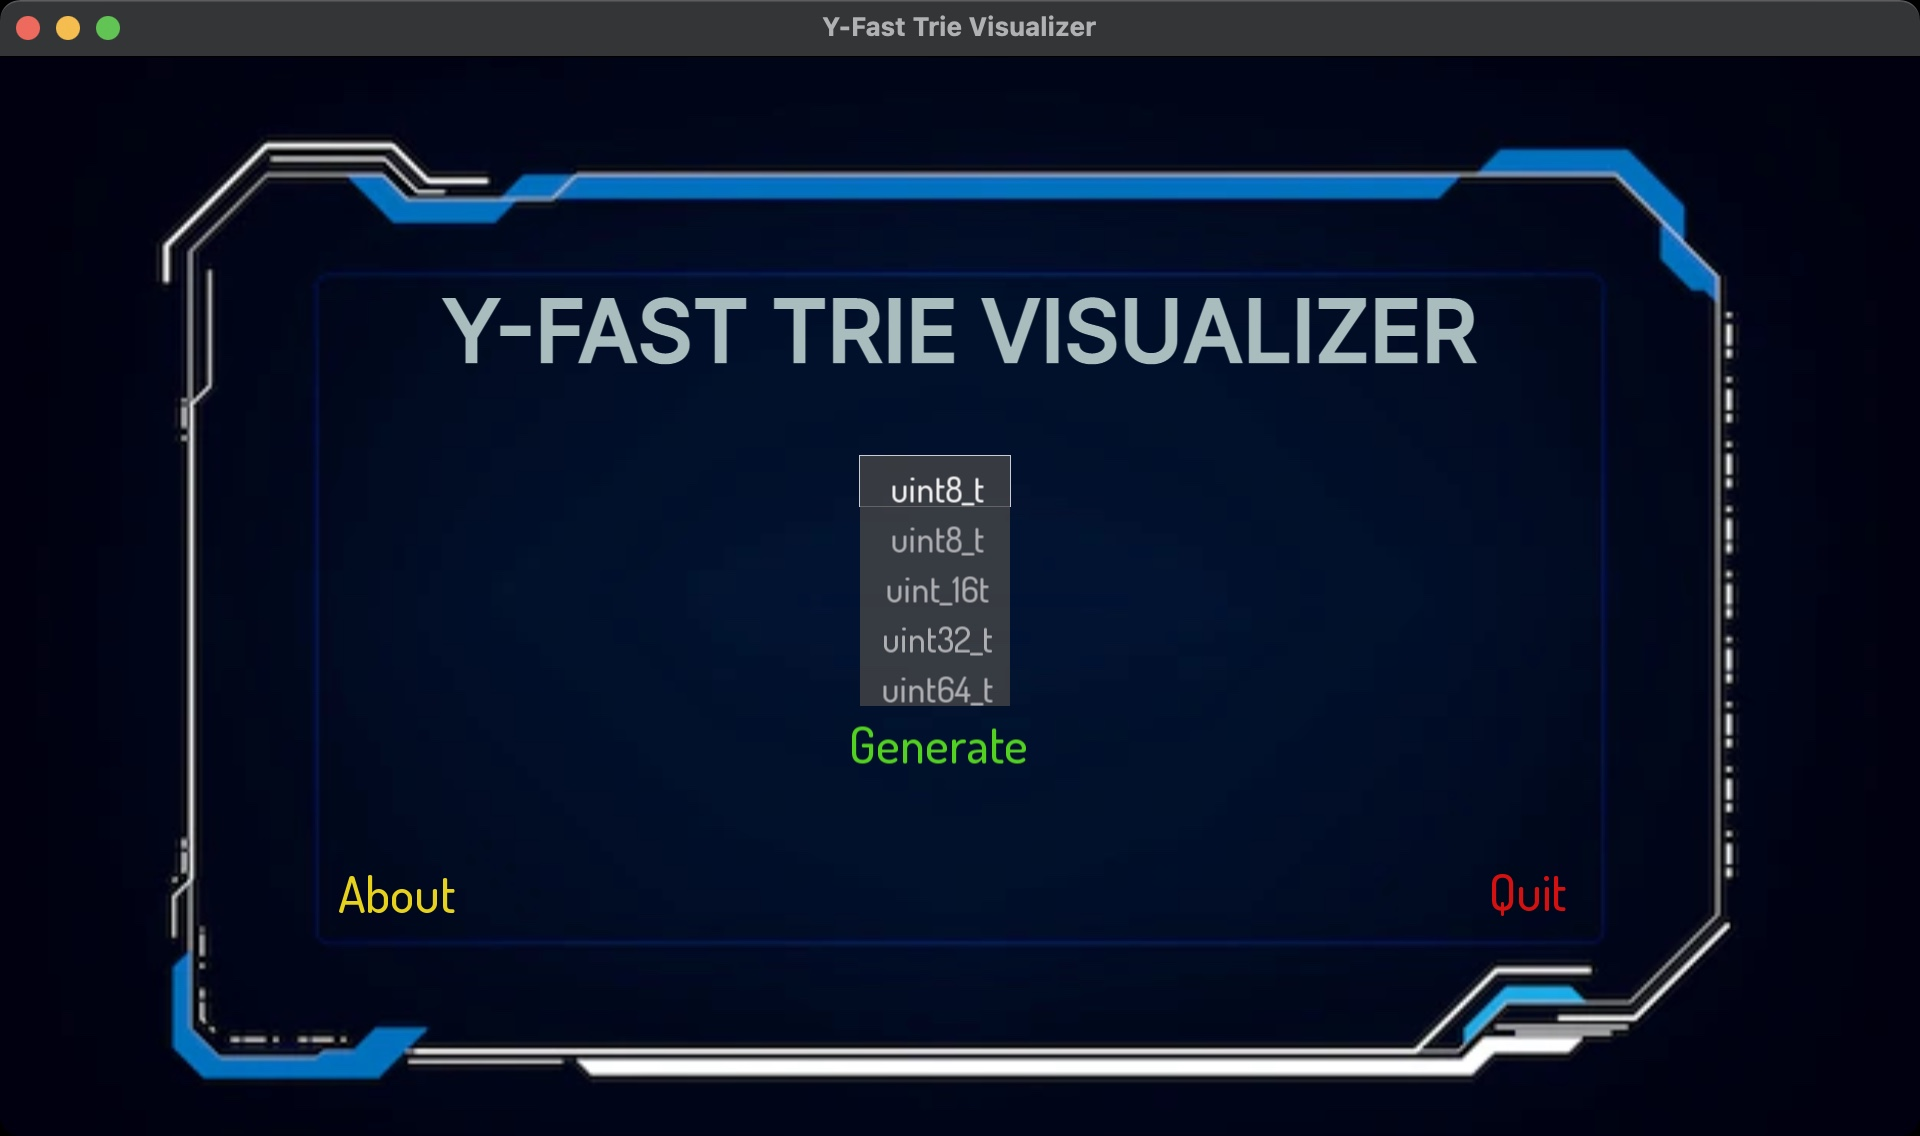
\includegraphics[width = 12cm]{mainmenu.png}
    \caption{The main menu state of the GUI}
\end{figure}

\subsubsection{About State}
The demo/states/about.h provides the user with a short description to familiarize the user with our project. Within this state is a “Go Back” button that will direct the user back to the main menu state. Additionally, this state contains a “Github” button that will open our git repository in the user’s default browser.

\begin{figure}[h]
    \centering
    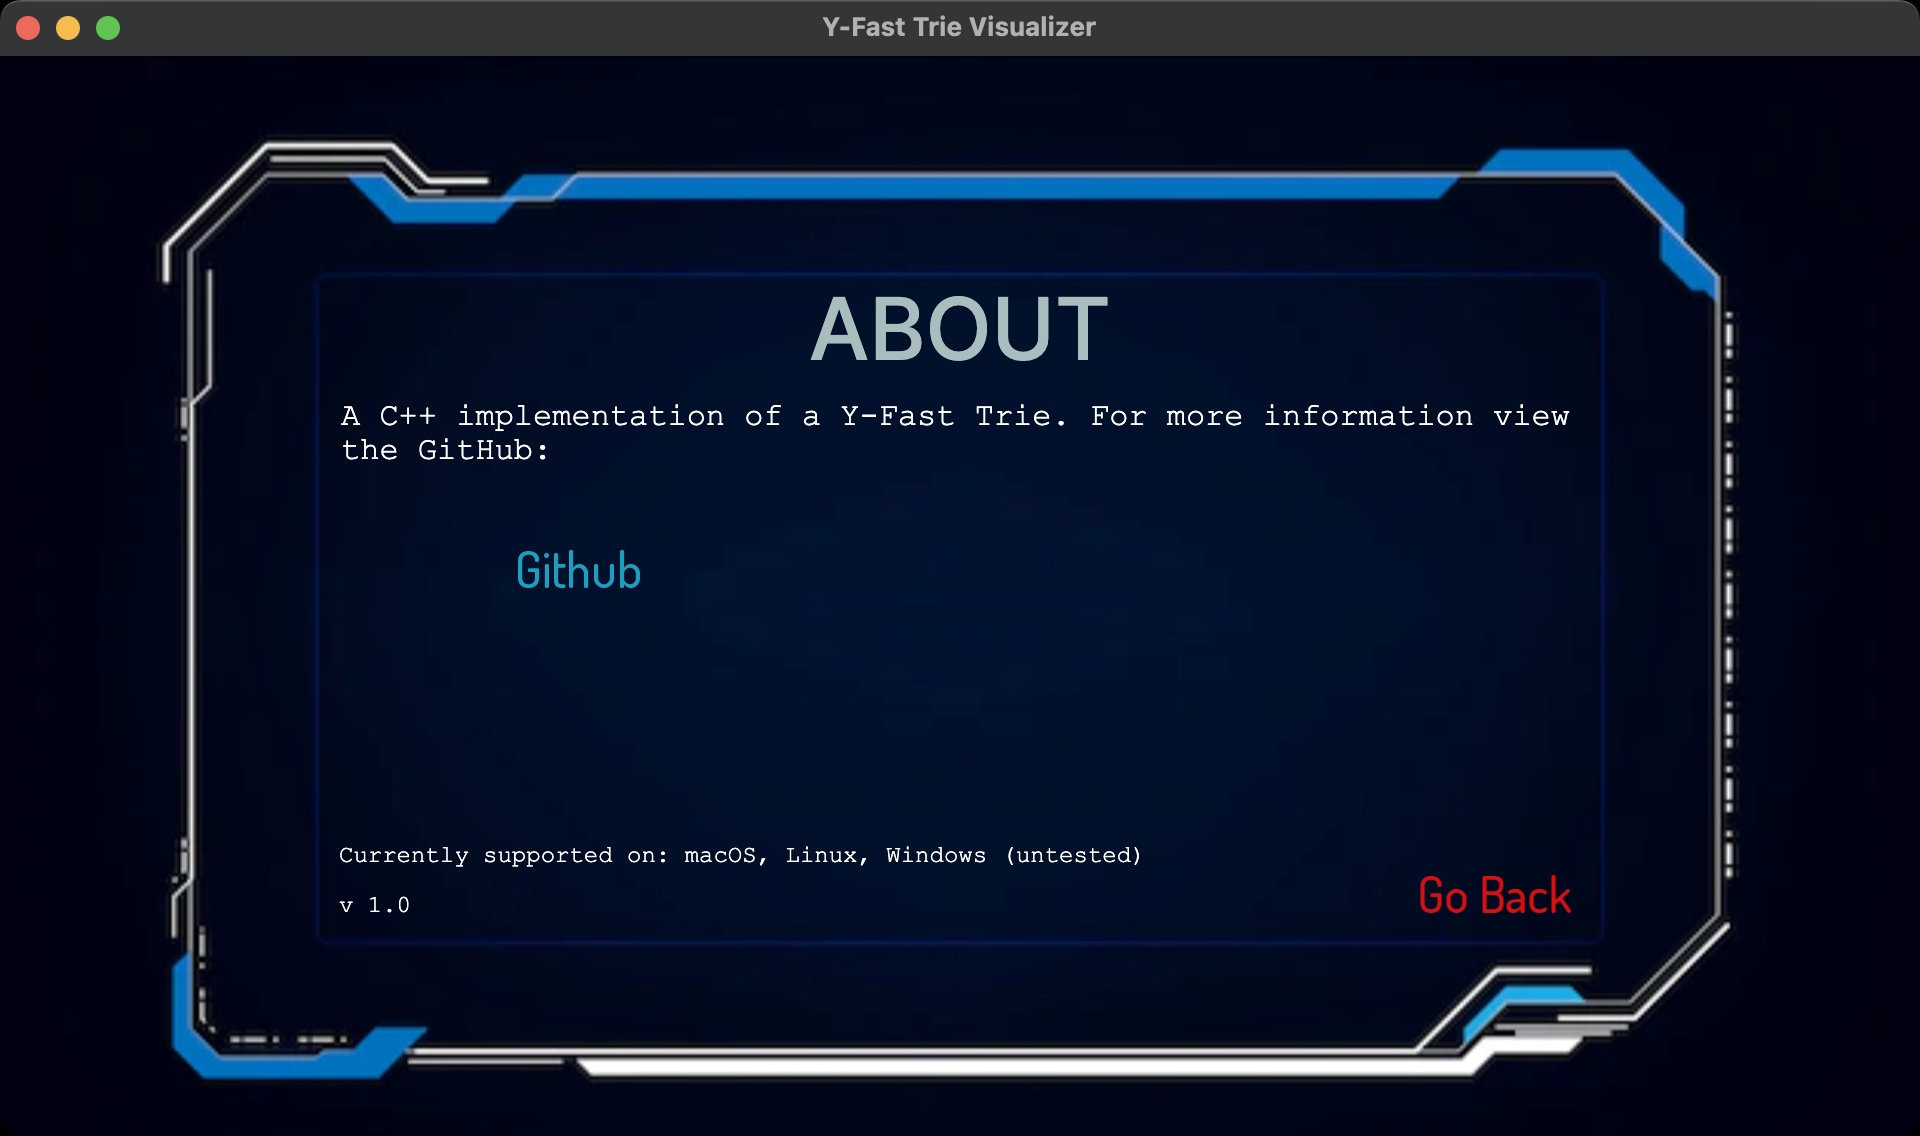
\includegraphics[width = 12cm]{github.png}
    \caption{The about state of the GUI}
\end{figure}

\subsubsection{Visualizer State}
The demo/states/visualizer.h is the primary state of the program as its function is to display the y-fast trie. This state has numerous features, such as keybinding support and a trie editor console, to enhance the user’s experience.
\\

\begin{figure}[h]
    \centering
    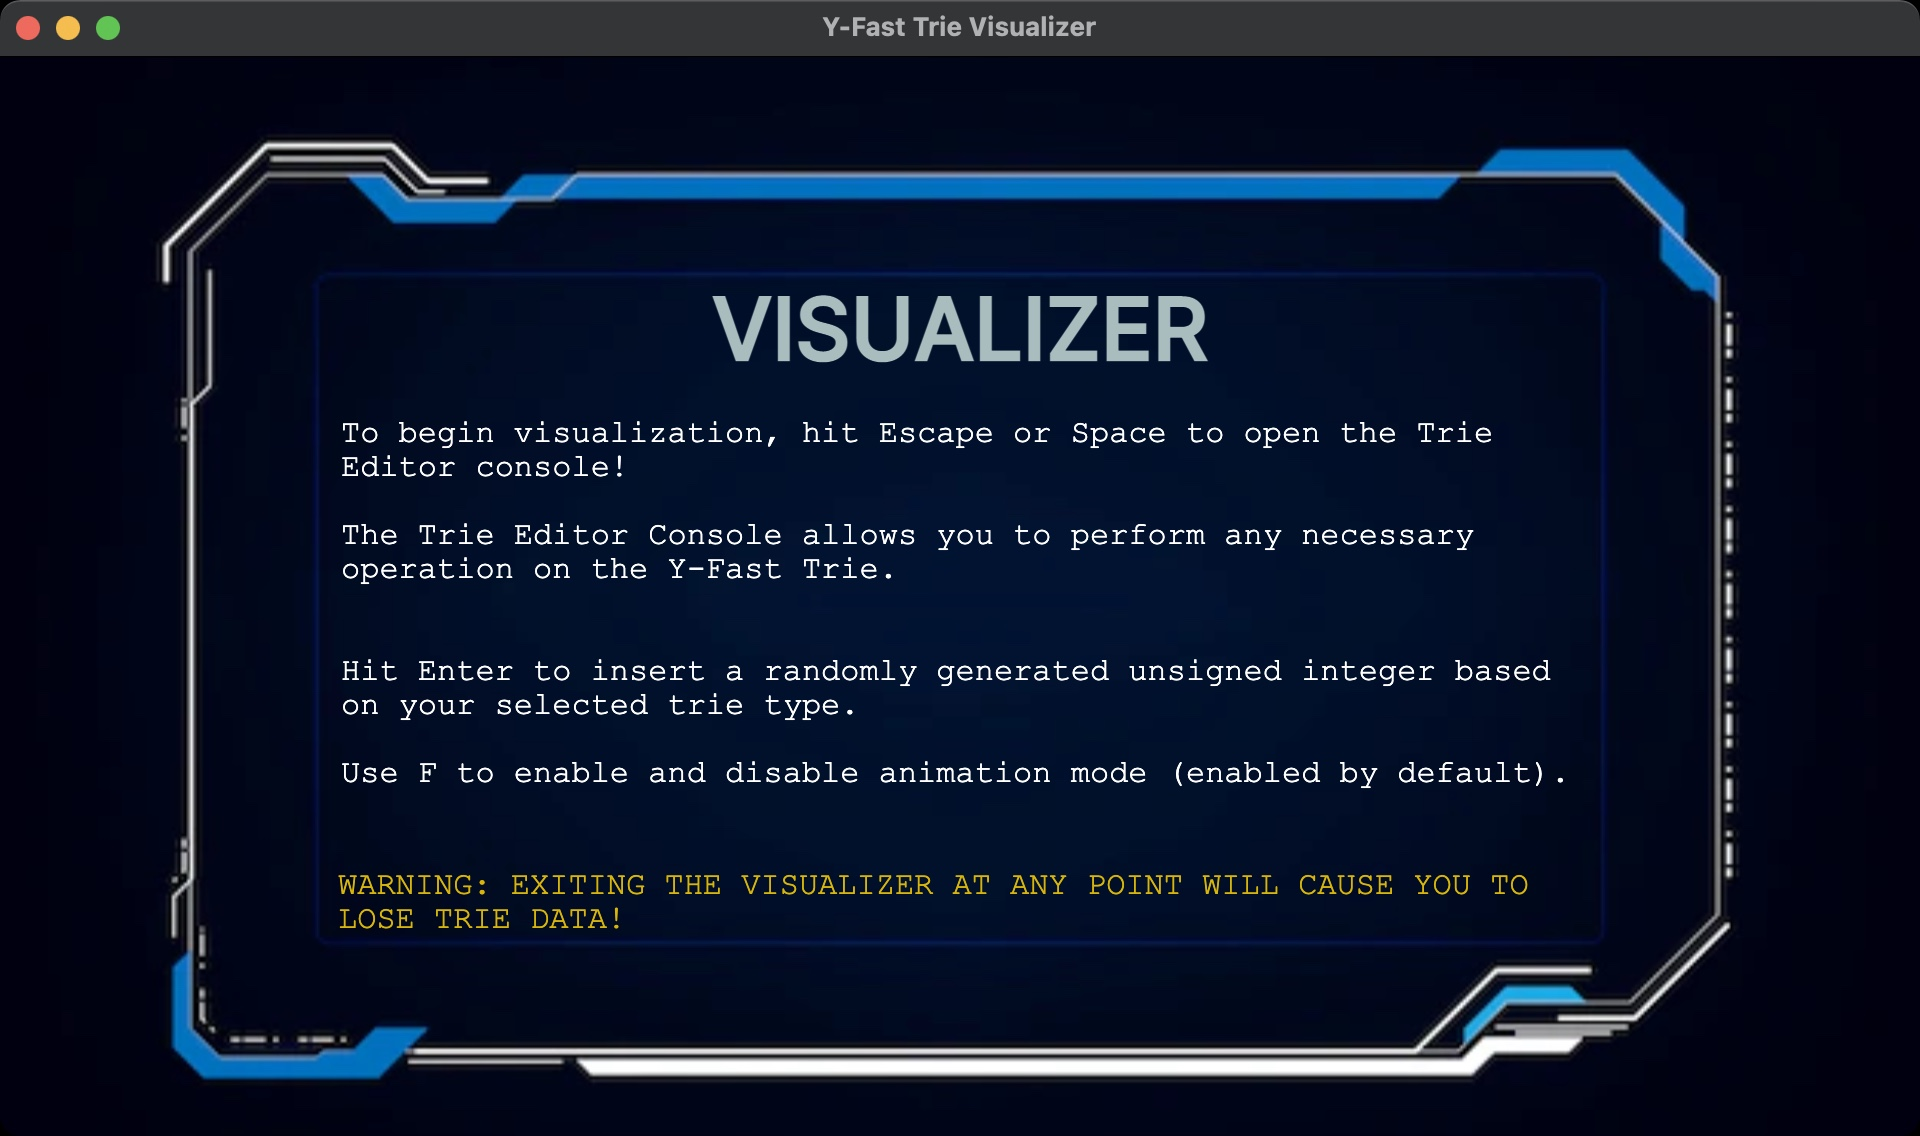
\includegraphics[width = 12cm]{tutorial.png}
    \caption{The visualizer state of the GUI}
\end{figure}

\noindent
The demo/tools/gui-.h and demo/tools/console.h are trie editor tools accessible only within this state which allow the user to perform numerous operations on the selected y-fast trie. The console accounts for inaccurate input. For example, if a value inserted is larger than the maximum of the selected unsigned integer type, the console replaces the insertion with the maximum value.

\begin{figure}[h]
    \centering
    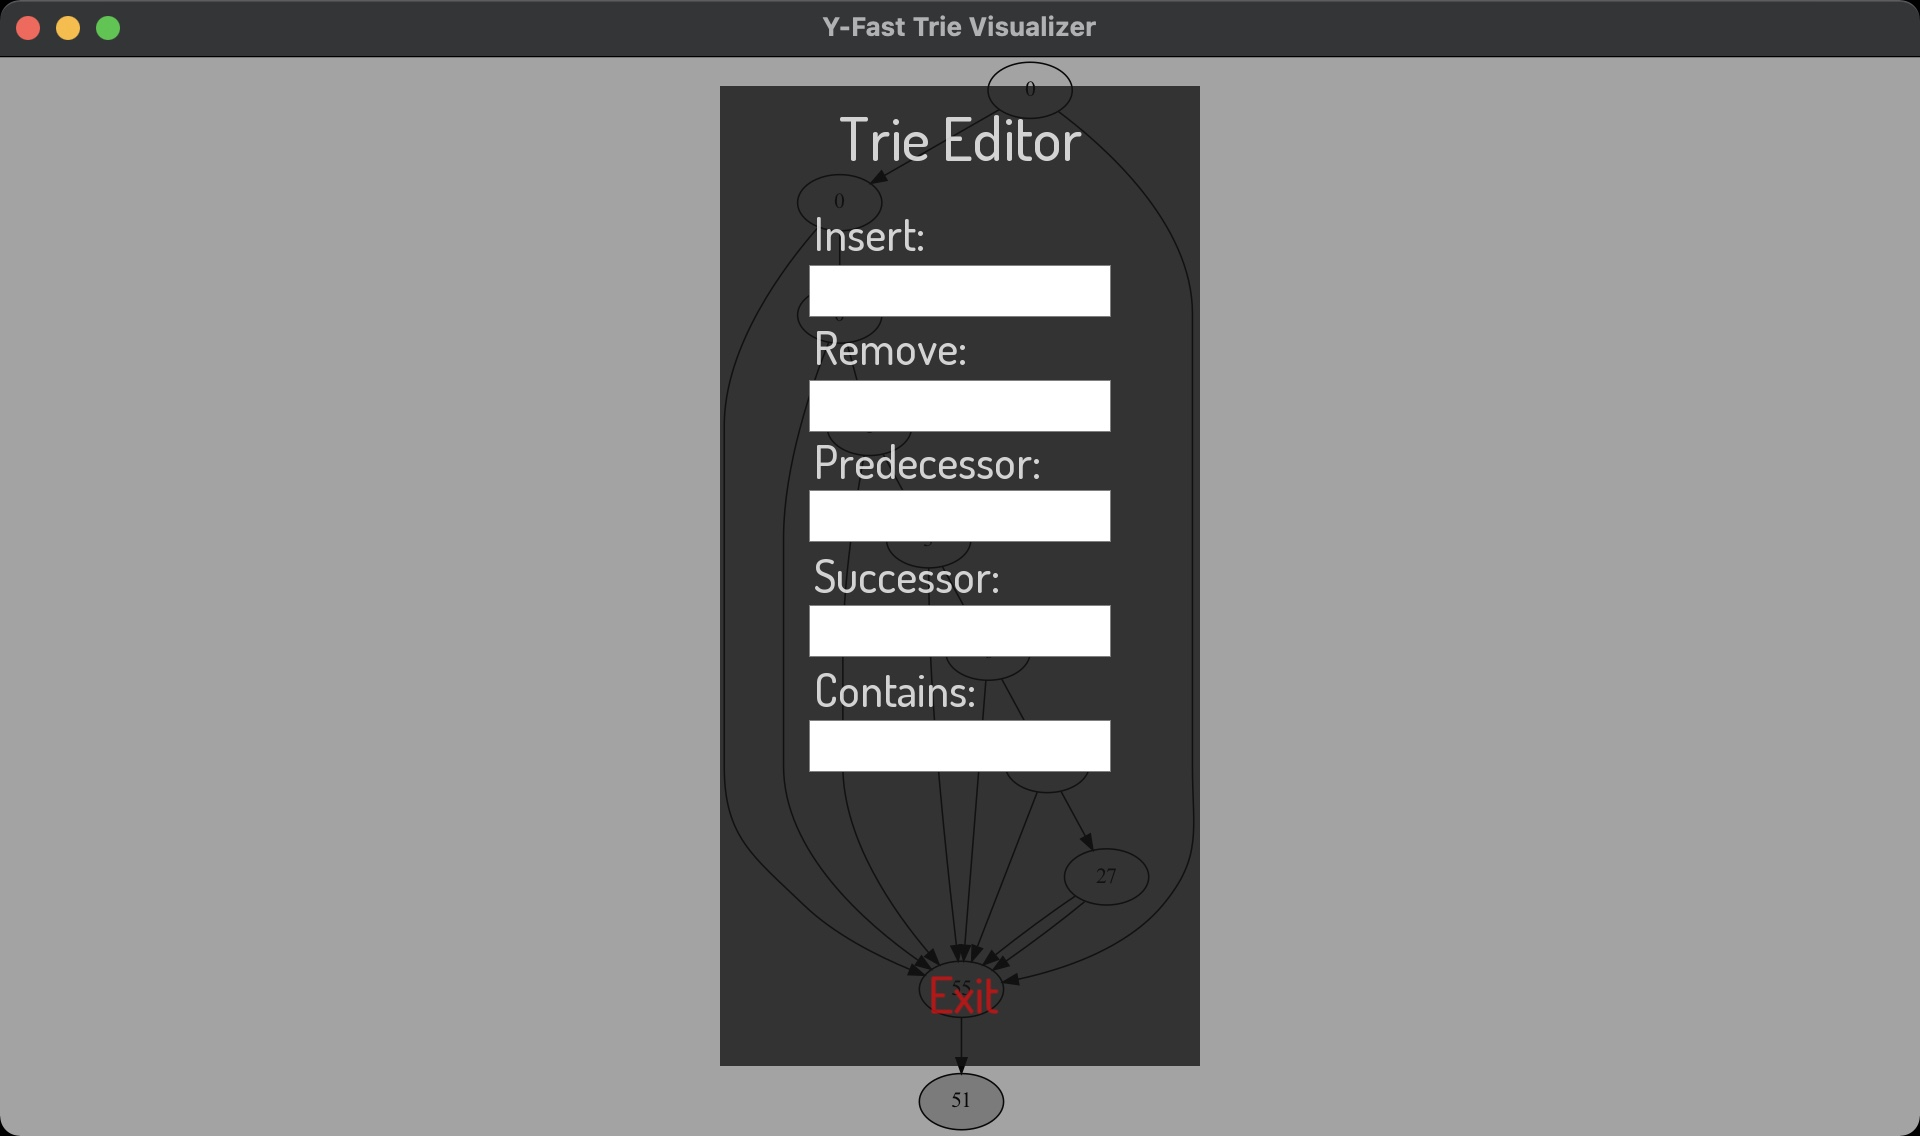
\includegraphics[width = 12cm]{input.png}
    \caption{The Trie Editor Console with all y-fast trie operations}
\end{figure}

\subsubsection{GUI Tools}
We developed a custom GUI tools library rather than using another GUI library. The demo/tools/gui-tools.h file contains the GUI tools used within this visualizer:

\begin{itemize}
    \item Button
    \item Drop-down List
    \item Text Box
\end{itemize}

A button is a tool that triggers an action when a user left-clicks within the bounds of the button. Buttons are used throughout the GUI as a method of traversing the various states of the program.
\\

\noindent
A drop-down list is a tool that is a collection of buttons. A user can select an item from the list by left-clicking within the bounds of the item. This will then change the first item to the one that was selected.
\\

\noindent
The text box provides the user with the ability to directly interact with the GUI. Once a textbox has been selected by left-clicking within the bounds of the text box, all other text boxes will no longer be available for selection. The user must provide input or exit the text box by entering with no input.
\\

\subsubsection{OS and Resolution Support}
The GUI is currently built to run on macOS, Linux, Windows (not officially unsupported) on a device that supports a 1920x1080 resolution.
The demo is run with the run.py script. This script executes the demo by adding the necessary SFML linker and includes paths to the command line.


\section{Results}
\noindent
We investigated 14 other open source implementations of y-fast tries. Due to time constraints, we were unable to benchmark against all implementations. We choose to only benchmark against the highest quality implementation due to Dinklage, Fischer and Herlez and std::set \cite{DBLP:journals/corr/abs-2104-06740}. Additionally, we benchmark both with a red-black tree for the partitions and a unsorted vector for the partitions. 
\\

\noindent
For the benchmark, we follow Dinklage, Fischer and Herlez's lead and perform $q$ insertions, $q$ predecessor queries then $q$ removals \cite{DBLP:journals/corr/abs-2104-06740}. 

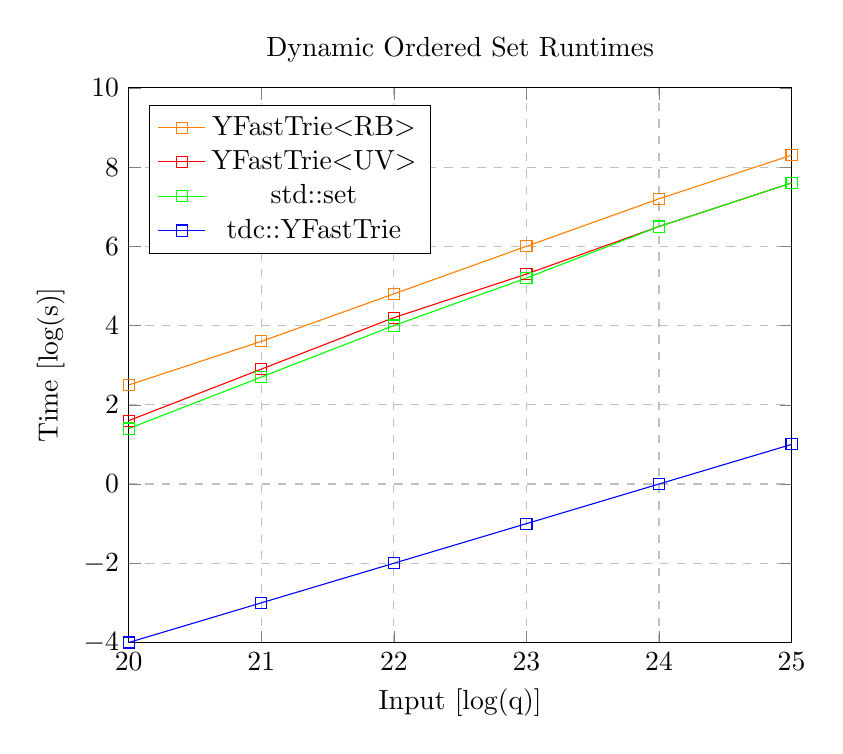
\begin{tikzpicture}
    \begin{axis}[
        title={Dynamic Ordered Set Runtimes},
        xlabel={Input [log(q)]},
        ylabel={Time [log(s)]},
        xmin=20, xmax=25,
        ymin=-4, ymax=10,
        xtick={20,21,22,23,24,25},
        ytick={-4,-2,0,2,4,6,8, 10},
        legend pos=north west,
        xmajorgrids=true,
        ymajorgrids=true,
        grid style=dashed,
    ]
    
    \addplot[
        color=orange,
        mark=square,
        ]
        coordinates {
        (20,2.5)(21,3.6)(22, 4.8)(23,6.0)(24,7.2)(25,8.3) 
        };
        \addlegendentry{YFastTrie\textless RB\textgreater}
     \addplot[
        color=red,
        mark=square,
        ]
        coordinates {
        (20,1.6)(21,2.9)(22,4.2)(23,5.3)(24,6.5)(25,7.6) 
        };
        \addlegendentry{YFastTrie\textless UV\textgreater}
    \addplot[
        color=green,
        mark=square,
        ]
        coordinates {
        (20,1.4)(21,2.7)(22,4.0)(23,5.2)(24,6.5)(25,7.6) 
        };
        \addlegendentry{std::set}
    \addplot[
        color=blue,
        mark=square,
        ]
        coordinates {
        (20,-4)(21,-3)(22,-2)(23,-1)(24,0)(25,1) 
        };
        \addlegendentry{tdc::YFastTrie}
    
    \end{axis}
\end{tikzpicture}

\noindent
We find that our implementation is nearly 100x slower than Dinklage, Fischer and Herlez's. We believe this is because we did not implement the level search structure optimization due to them. However, we outperformed std::set on very large inputs.

\section{Contributions}

\noindent
Calvin Higgins implemented the YFastTrie and XFastTrie. He also implemented the benchmarking and testing suites and investigated the performance of other implementations. He wrote the README and structured the project on GitHub. He wrote the X-Fast Trie and Y-Fast Trie sections of the report as well as the introduction, preliminaries, abstract and results section. He also created the presentation. Calvin created the run.py script.
\\

\noindent
Ethan Carlson implemented the RedBlackTree and wrote the Red-Black Tree section of the report. Calvin Higgins assisted in the implementation of some RedBlackTree methods, namely predecessor and successor. Calvin directly implemented O(n) split and merge. Calvin also made several tweaks for the final release of RedBlackTree.
\\

\noindent
Robert Oganesian implemented a BinarySearchTree and the demo program. He wrote the Demo section of the report. Robert wrote the installer script for MacOS and helped with the installer script for Linux. Robert also implemented the demo feature into run.py.

\section{References}
\printbibliography
\end{document}